% Made up for the tikra benchmark.
\usetikzlibrary{decorations.pathreplacing}
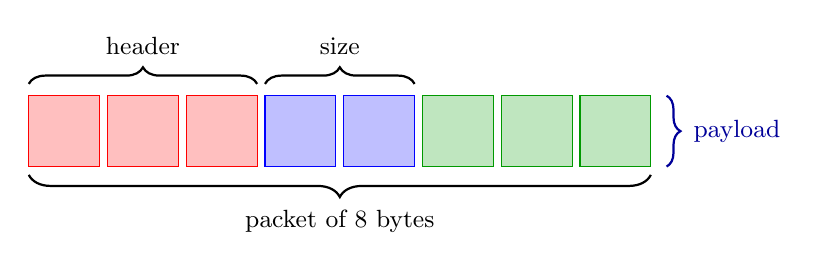
\begin{tikzpicture}[font=\small]
  \foreach \x/\c in {0/red, 1/red, 2/red, 3/blue, 4/blue, 5/green!60!black, 6/green!60!black, 7/green!60!black}
    \draw[fill=\c!25, draw=\c] (\x,0) rectangle +(0.9,0.9);
  \draw[decorate, decoration={brace, amplitude=6pt}, thick] (0,1.05) -- node[above=7pt] {header} (2.9,1.05);
  \draw[decorate, decoration={brace, amplitude=6pt}, thick] (3,1.05) -- node[above=7pt] {size} (4.9,1.05);
  \draw[decorate, decoration={brace, mirror, amplitude=8pt, raise=3pt}, thick] (0,0) -- node[below=12pt] {packet of 8 bytes} (7.9,0);
  \draw[decorate, decoration={brace, amplitude=5pt}, thick, blue!60!black] (8.1,0.9) -- node[right=6pt] {payload} (8.1,0);
\end{tikzpicture}
